\section{Kichererbsen Curry}
% Linke Seite: Rezept
Zutaten:
\begin{itemize}
    \item 1 Dose Kichererbsen (vorgekocht)
    \item 2 Paprika (rot und gelb)
    \item 1-2 Fenchel
    \item Zucchini (Wenn vorhanden)
    \item 1 Dose Kokusnusmilch
    \item 1 Dose Tomaten (oder entsprechende Menge frische Tomaten)
    \item 1 Strauch Frühlingszwiebeln
    \item (optional) 1 Dose Cashew-Nüsse
    \item 1 Glas rote Currypaste
\end{itemize}

\vspace{1cm}

\noindent Zubereitung:

\noindent Gemüse kleinschneiden. Kichererbsen abtropfen. Die Hälfte der
Currypaste in einer Pfanne (oder Wok) kurz anbraten, dann Gemüse hinzugeben und
zugedeckt bei mittlerer Hitze dünsten lassen. Nach etwa 10 Minuten Kichererbsen
dazu geben. Wenn das Gemüse den gewünschten Härtegrad hat, Kokusmilch
hinzugeben und aufkochen lassen. Mit Pfeffer und Salz abschmecken und mit Reis
servieren.

% Recht Seite: Bild
\newpage
\mbox{}
\vfill
\begin{center}
    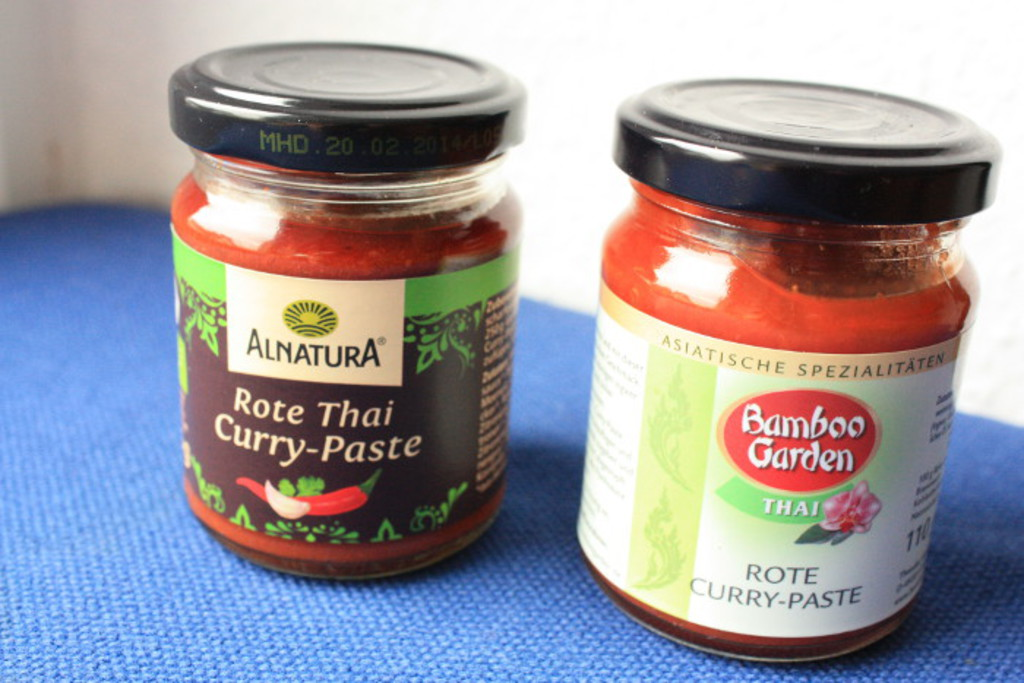
\includegraphics[width=0.5\textwidth]{Kichererbsen-Curry/IMG_6111_small.jpg}
\end{center}
\vfill
\begin{center}
    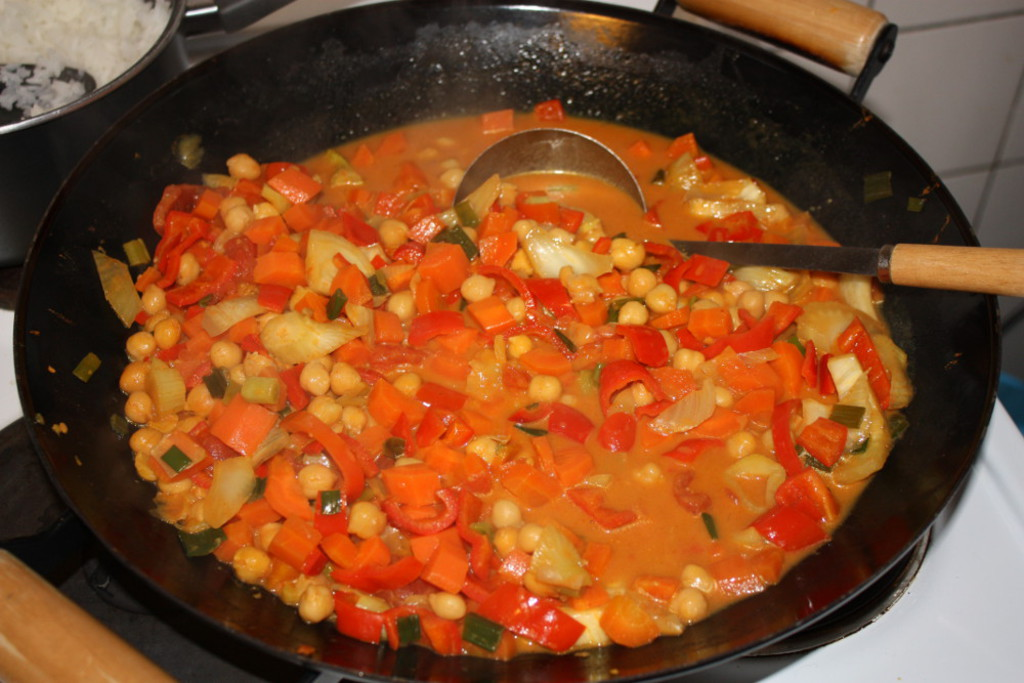
\includegraphics[width=\textwidth]{Kichererbsen-Curry/IMG_6085_small.jpg}
\end{center}
\vfill
\mbox{ }
\newpage
